\begin{quoting}
In this chapter we will have a closer look at different flour types
and their respective categorization. We will also look at common
ways to distinguish different flours of the same type. This way you can more confidently
purchase the flour that you need.
\end{quoting}

The most basic flour type is a whole grain flour. In this case the whole seed has
been grounded to smaller pieces. Sometimes, depending on what you want to bake,
the hearty taste of the bran might not be desired. In this case you can use
whiter flours. With sieves, mills remove larger parts of the hull of the seed.
The seed already contains a pre-built germ from the plant waiting to be
activated. The whitest flour you can get is mostly just the starch part of the seed.
Depending on which layers are still present, names are used to describe the
type of flour.

\begin{table}[!htb]
    \begin{center}
        \begin{tabular}{@{}llrrr@{}}
\toprule
\textbf{USA}  & \textbf{UK}  & {\textbf{Germany}} & {\textbf{France}} & {\textbf{Italy}} \\ \midrule
Cake         & Soft flour  &  T405    &  T45   & 00 \\ 
All purpose  & Plain flour &  T550    &  T55   &  0 \\ 
             &             &  T812    &  T80   &  1 \\ 
             &             & T1050    & T110   &  2 \\ 
Whole        & Whole       & Vollkorn & T150   & Integrale \\ \bottomrule
\end{tabular}

        \caption{A comparison of how different types of wheat flour are
        labelled in different countries.}%
        \label{tab:flour-types-comparison}
    \end{center}
\end{table}

In Germany, the ash content is used to describe the flours. The lab will burn
\qty{100}{\gram} of flour in the oven. Then afterwards the remaining ash is extracted
and measured. Depending on the quantity the flour is categorized. If the flour
is of type 405 then \qty{405}{\mg} of ash have remained after burning the
flour. The more hull parts the flour has, the more minerals remain. So the
higher the number, the closer the flour is to whole flour. The numbers are
slightly different between each grain type. Generally though, the higher the
value, the heartier the taste is going to be.

\begin{figure}[htb!]
  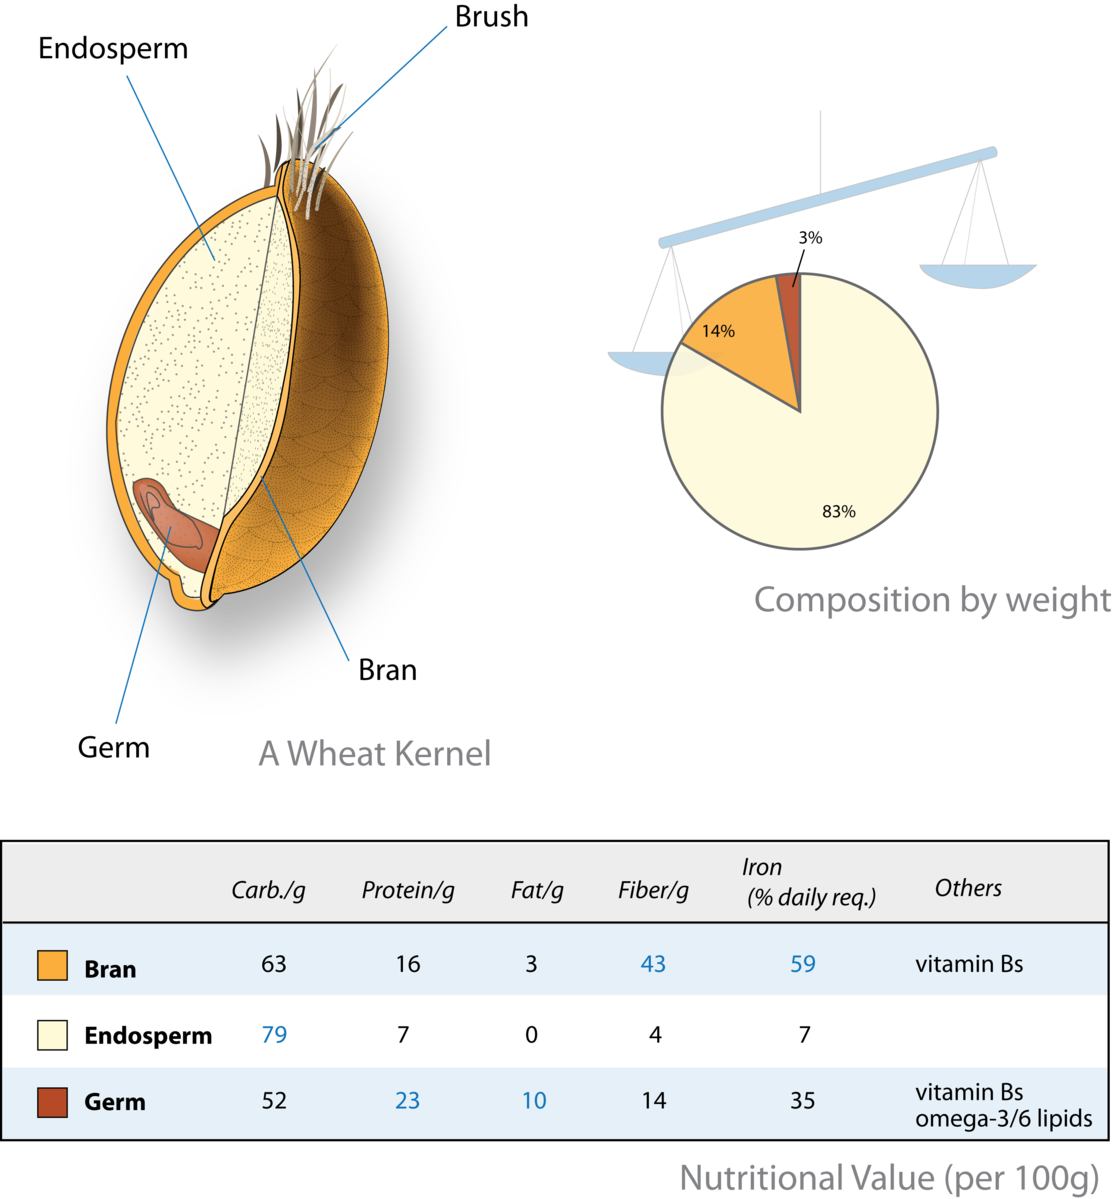
\includegraphics[width=\textwidth]{wheat-kernel-overview}
  \caption{An overview of a wheat kernel together with its
  content~\cite{wheat+kernel}.}%
  \label{fig:wheat-kernel-overview}
\end{figure}

If you compare different grain types, there are grains with high gluten, low gluten
and no gluten. Gluten is what enables bread to have its fluffy consistency.
Without gluten the baked goods wouldn't have the same properties. Managing
gluten makes the whole bread-making process more complex as more steps are involved.
A dough without gluten doesn't have to be kneaded. Kneading creates
the gluten bonds. The more you knead, the stronger they become. With low-gluten
and no-gluten flours, you only have to mix the ingredients together, making
sure you properly homogenize everything. During fermentation
the gluten degrades as the microorganisms metabolize it. When too much gluten
has been converted your dough will no longer have the wheat-like structure previously
described. For no/low gluten flour your main focus is managing acidity. You do not
want the final bread to be too sour. You do not have to worry about the gluten
degradation, removing a huge headache from the equation.

\begin{table}[!htb]
    \begin{center}
        \documentclass[tikz]{standalone}
\usepackage{tikz}
\usepackage{siunitx}
\DeclareSIUnit\degF{\text{°}F}

\begin{document}
\begin{tabular}{|l|l|l|l|l|}
\hline
\textbf{Grain type}              & \textbf{Homogenize} & \textbf{Knead} & \textbf{Stretch \& Fold} & \textbf{Shape} \\ \hline
\textbf{Wheat}                   & Yes                 & Yes            & Yes                      & Yes            \\ \hline
\textbf{\textgreater 70\% Wheat} & Yes                 & Yes            & Yes                      & Yes            \\ \hline
\textbf{Spelt}                   & Yes                 & Yes            & Yes                      & Yes            \\ \hline
\textbf{Rye}                     & Yes                 & No             & No                       & No             \\ \hline
\textbf{Emmer}                   & Yes                 & No             & No                       & No             \\ \hline
\textbf{Einkorn}                 & Yes                 & No             & No                       & No             \\ \hline
\textbf{Rice}                    & Yes                 & No             & No                       & No             \\ \hline
\textbf{Corn}                    & Yes                 & No             & No                       & No             \\ \hline
\end{tabular}
\end{document}

        \caption{An overview of different grain types and the steps involved
        in the respective bread making process.}
    \end{center}
\end{table}

As gluten has a special role, the rest of this chapter is dedicated to having a
closer look at different gluten flours and how to distinguish them. Spelt
also contains significant amounts of gluten, so the same characteristics hold
true.

Several recipes call for wheat bread flour. Bread flour can refer to different types
of flour. It could be a T405 or a T550 in Germany. This is very often
classified incorrectly. The terms \emph{strong} or \emph{bread} flour in this case
refer to the properties of the flour. A bread flour is considered to have a
higher amount of protein and thus gluten. This flour is excellent when you
want to make a sourdough bread as your dough allows for a longer leavening
period. As described earlier, the gluten is consumed by your microorganisms.
The more gluten you have, the longer your dough keeps its integrity. If you wanted
to make a cake, you might want to use a flour with less gluten. The gluten binding
properties might not be desirable since the final cake could have a chewy texture.

In conclusion, not every T405, T45 or T00 flour is the same. Depending on the properties
of the plant they come from, the flours will have different properties. For that reason
some countries like Germany have introduced additional scales to evaluate the quality of the
wheat. The category \textbf{A} refers to good quality wheat that can be blended
with poorer qualities to improve the flour. The category \textbf{B} refers to
average wheat that can be used to create different baked goods. Category \textbf{C}
is used for wheat that has poor baking qualities. This could happen, for instance,
if the wheat already started to sprout and thus lost some of its desirable
baking properties. This type of wheat is typically used in animal feed or
as fermentable biomass for generators. Category \textbf{E} refers to \emph{Elite} wheat. It's
the highest quality of wheat. This kind of wheat can only be harvested when the
wheat has grown under optimal conditions. You can compare this to a winery
that uses only the best grapes to make a reserve wine. Unfortunately, this is normally never printed
on the packaging of the flour that you buy. You can look out for the protein
value as a possible indicator. However, large mills blend flours together to
maintain quality throughout the years. Blended flour is also not listed on
the packaging. It might be that bakeries extract gluten from some flour and
then mix it in order to create better baking flours.

In Italy the so-called
\textbf{W-value} has been introduced to better show how the flour will behave.
A dough is made, and then the resistance of this dough to kneading is measured.
The more gluten a flour has, the more elastic the dough is, and the more it will
resist kneading. A higher W flour will have a higher gluten content and allow for a longer
fermentation period. But at the same time, it is also harder for the microbes to
inflate the dough as there is more balloon material. To make an excellent fermented
product out of a high W flour you will need to have a long fermentation period.
The long fermentation period also means that your microbes will enrich
your dough with more flavor.

\begin{table}[!htb]
    \begin{center}
        \begin{tabular}{@{}rcll@{}}
\toprule
\textbf{W-Value} & \textbf{Hydration (\%)} & \textbf{Uses} & \textbf{Fermentation time} \\ \midrule
0--150          & 50     & Cookies             & Very short    \\ 
150--250        & 50--60 & Cakes, Bread, Pizza & Short--Medium \\ 
250--350        & 60--70 & Bread, Pizza        & Long          \\ 
350+            & 70--90 & Bread, Pizza        & Very long     \\ \bottomrule
\end{tabular}

        \caption{An overview of different levels of W values and the
        respective hydrations and fermentation times.}%
        \label{tab:w-value}
    \end{center}
\end{table}

Generally, when aiming to
bake free standing sourdough bread, aim for a higher protein content. If the
gluten value is relatively low, your bread will collapse faster. Baking bread
is still possible, but it might be easier to use tools such as a loaf pan, or
to make skilled bread or flatbread.

An additional, rarely considered characteristic of good flour is the level of damage to the
starch molecules. This is a common problem when you are trying to mill your own wheat flours at
home. The chances are that your home mill is not able to achieve the same results
a larger mill can. The damaging of the starches is essential to improve the
properties of the dough. You will have better gelatinization and water
absorption with properly damaged starch~\cite{starch+damage+flour}. As more
starch is damaged, the surface area increases. This improves how water interacts with the flour.
This also provides a larger surface that your microbes can use to attack the molecules
and start the fermentation process.

I~am still
yet to find a good way of milling my own flour at home. Even after trying to
mill the flour 10 times with short breaks, I~was not able to achieve the same
properties as with commercially milled flour. The doughs I~would make felt
good, maybe a bit coarse. However, during baking the doughs would start to
de-gas quickly and turn into very flat breads. I~have had great success though when
utilizing home-milled flour together with a loaf pan or as a pan bread. If you
have found great ways to work with home-milled flour, please reach out. The potential
of using home-milled flours is huge. It would enable even distant communities
to grow their own wheat and be able to produce amazing freshly baked bread.
